%!TEX TS-program = xelatex 
%!TEX TS-options = -output-driver="xdvipdfmx -q -E"
%!TEX encoding = UTF-8 Unicode
%
%  summary_2
%
%  Created by Mark Eli Kalderon on 2009-01-25.
%

\documentclass[11pt]{article} 

% Definitions
\newcommand\myauthor{Mark Eli Kalderon} 
\newcommand\mytitle{Oxford Philosophy of Perception:}
\newcommand\mysubtitle{Cook Wilson on Visual Extension and Appearance}

% Packages
\usepackage{url}
\usepackage{txfonts}
\usepackage{color}
\definecolor{myblue}{rgb}{0.8,0.8,1}

% Define discussion environment
\makeatletter\newenvironment{discussion}{%
   \noindent\begin{lrbox}{\@tempboxa}\begin{minipage}{\columnwidth}\setlength{\parindent}{1em}}{\end{minipage}\end{lrbox}%
   \colorbox{myblue}{\usebox{\@tempboxa}}
}\makeatother

% XeTeX
\usepackage[cm-default]{fontspec}
\usepackage{xltxtra,xunicode}
\defaultfontfeatures{Scale=MatchLowercase,Mapping=tex-text}
\setmainfont{Hoefler Text}
\setsansfont{Gill Sans}
\setmonofont{Inconsolata}

% Title Information
\title{\mytitle\\
\mysubtitle}
\author{\myauthor} 
\date{} % Leave blank for no date, comment out for most recent date

% PDF Stuff
\usepackage[plainpages=false, pdfpagelabels, bookmarksnumbered, backref, pdftitle={\mytitle}, pagebackref, pdfauthor={\myauthor}, xetex, colorlinks=true, citecolor=gray, linkcolor=gray, urlcolor=gray]{hyperref}

%%% BEGIN DOCUMENT
\begin{document}

% Title Page
\maketitle

% Layout Settings
\setlength{\parindent}{1em}

% Main Content

\begin{figure}[htbp]
	\centering
		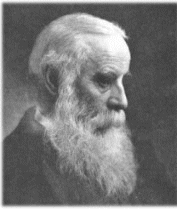
\includegraphics[scale=1]{../../graphics/wilson.jpg}
	\caption{John Cook Wilson}
	\label{fig:wilson}
\end{figure}

\section{Preliminaries}\label{sec:preliminaries} % (fold)

According to Stout, while there is a genuine explanatory distinction between primary and secondary qualities, there is more in common between primary and secondary qualities than is claimed by the Lockean view (as understood by Locke and his modern followers). Specifically, primary and secondary qualities are in one way dependent on sensation and in one way independent of sensation:
    \begin{itemize}
        \item They are each dependent on sensation in that they inherit their qualitative character from the character of the sensation but only insofar as that sensation is representative of something else.
        \item They are each independent of sensation in that objects may instantiate primary and secondary qualities independently of being perceived.
    \end{itemize}

Cook Wilson's criticism of Stout is focused on the dependency thesis and the representative realism that it presupposes. His critique is organized around three sets of considerations of increasing generality:
    \begin{enumerate}
        \item Criticism of visual extension (the sensation involved in the visual perception of extension)
        \item Criticism of Stout's understanding of apparent size that motivates the postulation of visual extension
        \item A fundamental diagnosis of this in terms of a conflation of different senses of appearance talk.
    \end{enumerate}

% section preliminaries (end)

\section{Visual Extension}\label{sec:visual_extension} % (fold)

Concerning Stout's distinction between visual extension and real extension Cook Wilson makes four sets of remarks. The discussion builds on his discussion of representation. He emphasizes that the sense-representation differs in kind from what it represents. That the sense-representation is numerically distinct directly follows from Stout's representative realism, that sense-representation mediates our knowledge of what it represents. Cook Wilson, however, is relying on the stronger claim that sense-representation and what it represents are not only numerically distinct, but distinct in kind. So far, Cook Wilson has offered two reasons for this further claim:
    \begin{enumerate}
    	\item The Berkelean reasoning: Only a sensation can resemble a sensation. So if representation were mimetic, the plain man would be committed to the ``flagrant absurdity'' that sensations can exist and change unperceived.
    	\item The phenomenological claim that there is nothing in sensation which is spatial
    \end{enumerate}

The four set of remarks:

A. Given the Berkelean reasoning, visual extension represents something unlike itself, so real extension differs in kind from any figure that is presented to us in perception or visual imagination. What, then, is real extension? We cannot say. Stout is ``committed to something worse even than a `thing in itself', viz., to `an attribute in itself'''.

B. That real extension is of the same kind as visual extension presupposed by the science of geometry. Two considerations:
    \begin{enumerate}
    	\item Just as there could be no science of a thing in itself, there could be no science of extension of itself.
	    \item Constructive proofs in geometry presuppose that extension presented in perception and visual imagination is real extension.
    \end{enumerate}

C. The phenomenological difference between heat and color. The sensation of heat is felt in the affected part of the body. We experience color, in contrast, as clearly and distinctly located in the perceived external object. (This is the phenomenological difference that is reflected in ordinary language.) It follows that color cannot be representative of extension because we cannot perceive it except as extended---as inhering in an extended surface. Nor can we imagine otherwise. If we perceive color, we must perceive at the same time extension. Cook Wilson supports this by observing that if we perceive adjacent homogenous colors we necessarily perceive their boundary.

D. If sensation is extended, then sensible extension (the sensation, whether tactual or visual, involved in the perception of extended bodies) is merely subjective. That sensible extension is merely subjective is absurd (committed to attributes in themselves, the impossibility of the science of geometry, and flouts phenomenology). Therefore no sensation, whether tactual or visual, could be extended.

E. 

The conclusion: Sensations are not extended and the idea of extension is \emph{absolutely inapplicable} to them.

% section visual_extension (end)

\section{Apparent and Real Size}\label{sec:apparent_and_real_size} % (fold)

Cook Wilson claims that Stout gets confused about visual extension because of his understanding of the distinction between real and apparent size. 

Cook Wilson's methodology here anticipates Austin:

    \begin{quote}
    	Just as ``representative and represented'' so ``real and apparent'' seem to me regular trap words, which cannot be safely used in any particular case without a most patient examination of their meaning and justification in the particular instance.
    \end{quote}

Cook Wilson makes negative and positive remarks about real and apparent size.

\subsection{Negative Remarks}\label{sub:negative_remarks} % (fold)

A. Stout's theory seems committed to a form of subjective idealism:

    \begin{enumerate}
    	\item Sensible extension is not real extension since real extension is in space but sensible extension is not. (By hypothesis, for the sake of reductio)
	    \item Things appear extended in space.
	    \item The space in which things appear extended is not real.
	    \item This seems to be committed to a form of subjective idealism.
    \end{enumerate}
    
B. Cook Wilson's strategy is to argue against Stout's claim that real and apparent size are incommensurable and then to draw out some implausible consequences from what remains of his view. First apparent size and real size must be commensurable. If apparent size is a \emph{size}, it has a measure. There must then be a common measure between real and apparent size. This seems implausible. The reasoning overgeneralizes. There would be no incommensurable measures, but there are. 

Cook Wilson however has an interesting subsidiary argument. How do we measure the real extension of a line. Well, you use a ruler. But by hypothesis it is the merely apparent extension of the ruler which is given in experience. You might think that we apply the visual extension of the ruler to the apparent line. But this presupposes that real extensions are in the same ratio to one another as apparent extensions. (And hence real and apparent size are commensurable.) 

But, further, how do we know that real and apparent extension are in proportion since real extensions are never the objects of perception. Supposing that real and apparent size are commensurable. Since apparent size varies with distance there must be some distance in which real and apparent size coincide. But what distance is that?

% subsection negative_remarks (end)

\subsection{Positive Remarks}\label{sub:positive_remarks} % (fold)

Two things can be equal in size and yet one can look smaller than the other because it is further from the viewer than the other. How are we to understand the sense in which it ``looks smaller''. Cook Wilson is, at this point, satisfied that understanding the apparent size of the thing cannot be understood as something which is both subjective and the object of experience. He thus seeks to understand the thing's looking smaller as some objective feature of the thing by drawing on some elementary features of classical perspective. Indeed his account turns on the observation that motivates classical perspective---that we cannot see around colors. ``The observer sees a point in the real extension of a real object in the direction (real) of the line drawn from his eye in real space to the given point in the real object''.

% subsection positive_remarks (end)

% section apparent_and_real_size (end)

\section{A Confusion about Appearance}\label{sec:a_confusion_about_appearane} % (fold)



% section a_confusion_about_appearane (end)

\end{document}
